\documentclass[a4paper]{article}

\usepackage[utf8]{inputenc}
\usepackage[portuges]{babel}
\usepackage[T1]{fontenc}
\usepackage{graphicx}
\usepackage{a4wide}
\usepackage[pdftex]{hyperref}
\usepackage{float}
\usepackage{indentfirst}
\usepackage{subcaption}

\begin{document}

\title{\textbf{Controlo e Monitorização de Processos e Comunicação}\\Trabalho Prático\\ Sistemas Operativos\\Grupo 22}
\author{Carlos Gomes (a77185) \and Márcia Teixeira (a80943) \and Rui Armada (a90468)}
\date{\today}

\begin{titlepage}

  %título
  \thispagestyle{empty}
  \begin{center}
  \begin{minipage}{0.75\linewidth}
      \centering
  %engenharia logo
      
\includegraphics[width=0.4\textwidth]{eng.jpg}\par\vspace{1cm}
      \vspace{1.5cm}
  %titulos
      \href{https://www.uminho.pt/PT}{\scshape\LARGE Universidade do Minho} \par
      \vspace{1cm}
      \href{https://www.di.uminho.pt/}{\scshape\Large Departamento de Informática} \par
      \vspace{1.5cm}

  \maketitle
  \end{minipage}
  \end{center}

  \clearpage

 \end{titlepage}
 
 \begin{abstract}

O presente documento descreve o trabalho prático realizado no âmbito da disciplina de
\href{http://miei.di.uminho.pt/plano_estudos.html#sistemas_operativos}
{\emph {Sistemas Operativos} (SO)}, ao longo do segundo semestre,
do segundo ano, do \href{http://miei.di.uminho.pt}{Mestrado Integrado em Engenharia Informática}
da \href{https://www.uminho.pt}{Universidade do Minho}.

O objetivo deste projeto foi desenvolver um serviço de monitorização de execução e de comunicação entre processos que permita a um utilizador fazer a submissão de sucessivas tarefas, tarefas das quais serão enviadas para um servidor que as vai executar e apresentar várias funcionalidades tais como: Se a tarefa foi efetuada com sucesso, mostrar o histórico de todas as tarefas feitas, etc.

Neste relatório iremos descrever com clareza todo o raciocínio e decisões tomadas ao longo da elaboração deste projeto.

\end{abstract}

\pagebreak

\tableofcontents

\pagebreak
\section{Introdução}
\label{sec:intro}

O objetivo deste projeto é implementar um serviço de gestão de processos de forma a ser capaz de monitorizar a execução e comunicação entre processos. Para implementarmos este serviço, iremos implementar uma arquitetura Cliente, Servidor, com recurso a pipes e aplicar outros conhecimentos acumulados ao longo da unidade curricular de Sistema Operativos. 



\subsection{Objetivo}
\label{sec:objetivo}

Como foi referido anteriormente, um dos objetivos deste serviço é a monitorização de execução e comunicação entre processos, onde o serviço deverá permitir a um utilizador a submissão de tarefas em que cada uma delas será uma sequência de comandos encadeados por pipes. 
Para além de iniciar as tarefas, o serviço também deverá ser capaz de identificar quais são as tarefas em execução, assim como terminar essas mesmas. 
Também deverá oferecer uma interface ‘amigável’ para o utilizador, onde o utilizador irá executar os comandos e visualizar a execução dessas tarefas.



\section{Conceção da Solução}
\label{sec:solução}
No sentido de resolver a problemática apresentada foi necessário partir do princípio que o problema inicial teria de ser dividido em problemas mais pequenos.\bigskip

Numa primeira fase foi idealizada a estrutura que viria a ter tanto o servidor como o cliente. Para tal, e sabendo que iriam comunicar através de pipes (com nome), foi tomada a decisão que o servidor apenas teria controlo sobre um pipe inicialmente criado para assegurar que o processo de conexão com um cliente decorreria normalmente. A função deste pipe será a transmissão dos nomes dos pipes, posteriormente utilizados para a comunicação dos pedidos do cliente, ao servidor e consequente resposta aos mesmos.
No sentido de evitar colisões nos pipes utilizados para envio de mensagens entre cliente e servidor, cada cliente que efetua uma nova conexão com o servidor cria os seus próprios pipes de leitura e de escrita, que diferem de todos os outros clientes à exceção do sufixo “-in” e “-out”, respetivamente. Assim garante-se que dois clientes distintos não lêem informações um do outro, permitindo que vários estejam ativos em simultâneo, apesar de se poderem encontrar bloqueados à espera de serem atendidos pelo servidor.\bigskip

Tendo ficado tratado o ponto indispensável do presente projeto, que é a comunicação, passou-se então a uma segunda fase, que seria o desenvolvimento das funcionalidades enunciadas para o funcionamento mínimo do sistema.
Já fazendo referência ao cliente singular, foi desenvolvido apenas um sistema básico de leitura de texto e envio para o servidor, que por sua vez tomará conta dos pedidos e é responsável pela resposta de acordo com a usabilidade do input recebido.
Por sua vez, o servidor desenvolvido trata-se do sistema mais complexo e portanto mais ponderado do projeto, pelas várias funções que desempenha no mesmo.



\pagebreak

\section{Implementação}
\label{sec:implementação}
\subsection{Cliente -> Servidor}
Para o desenvolvimento do serviço, é crucial haver uma comunicação entre o servidor e o cliente. O utilizador poderá agir sobre o servidor através dos argumentos passados na linha de comando do cliente e o servidor deverá receber esses argumentos e executar de acordo com o desejo do cliente.

\begin{figure}[H]
\centering
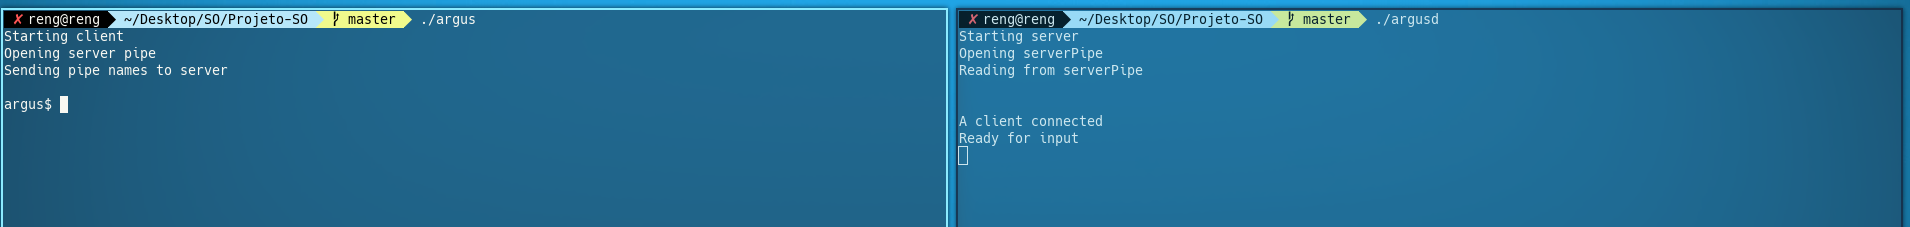
\includegraphics[scale=0.2]{SO1.png}
\caption{Cliente->Servidor}
\label{img:Ligação Cliente->Servidor}
\end{figure}

\section{Funcionalidades}
\label{sec:funcionalidades}
Como já foi referido anteriormente, é pretendido o desenvolvimento de um serviço de monitorização de execução e comunicação de processos. Então para isto acontecer, é necessário a existência de algumas funcionalidades que iremos explorar.
\subsection{\textbf{Execução de Tarefas}}
Funcionalidade que executa uma tarefa.
\begin{figure}[H]
\centering
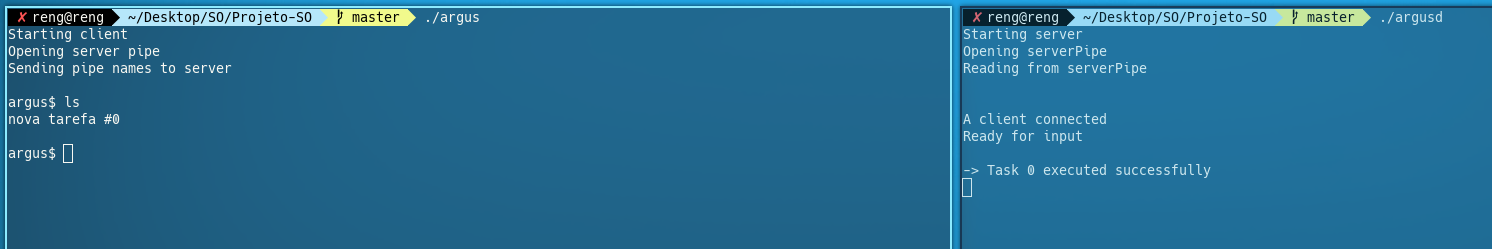
\includegraphics[scale=0.3]{SO2.png}
\caption{Execução de Tarefas}
\label{img:Execução de Tarefas}
\end{figure}

\subsection{\textbf{Mostrar o resultado da execução de tarefas}}
Fumcionalidade para consultar o \textit{standard output} produzido por uma tarefa ja executada.
\begin{figure}[H]
\centering
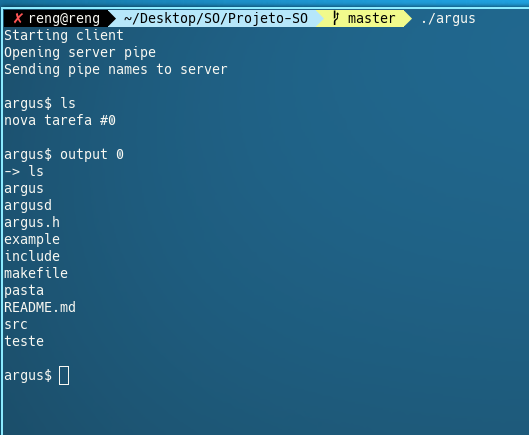
\includegraphics[scale=0.4]{SO3.png}
\caption{Mostrar o resultado da execução de tarefas}
\label{img:Mostrar o resultado da execução de tarefas}
\end{figure}

\subsection{\textbf{Definição de tempo de execução}}
Funcionalidade que fornece o tempo maximo (segundos) de execução de uma tarefa.
\begin{figure}[H]
\centering
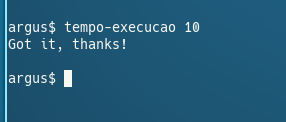
\includegraphics[scale=0.7]{SO4.png}
\caption{Definição de tempo de execução}
\label{img:Definição de tempo de execução}
\end{figure}

\subsection{\textbf{Mostrar que só pode executar um programa em n segundos}}
Funcionalidade que obriga a execução de um programa num dado periodo de tempo defenido pelo Utilizador.
\begin{figure}[H]
\centering
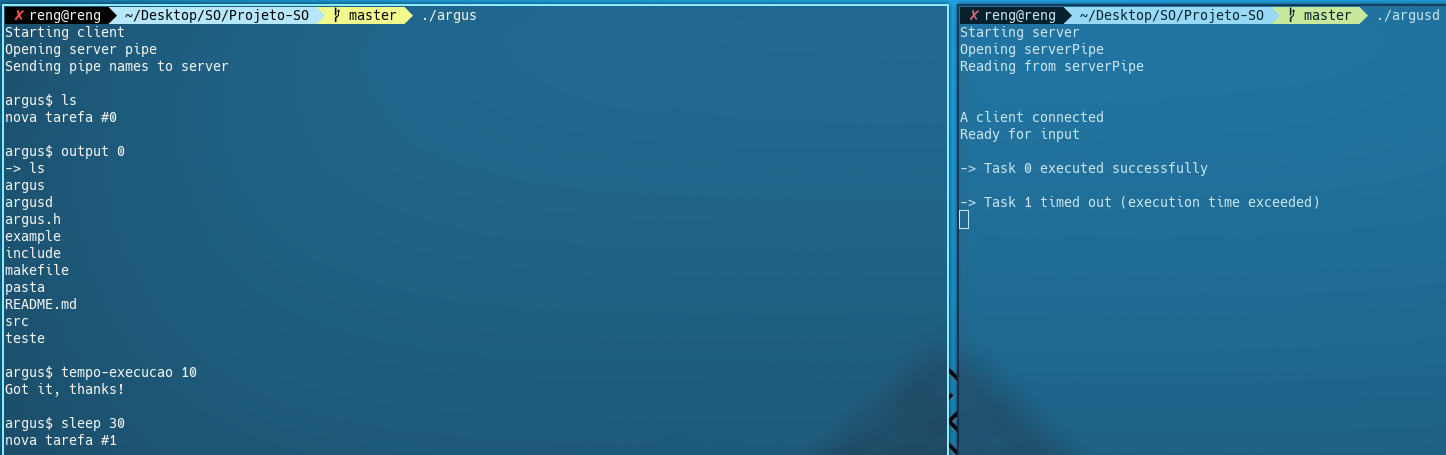
\includegraphics[scale=0.3]{SO5.png}
\caption{ Mostrar que só pode executar um programa em n segundos}
\label{img: Mostrar que só pode executar um programa em n segundos}
\end{figure}

\subsection{\textbf{Ajuda}}
Funcionalidade que apresenta o menu de ajuda para a Utilização da Aplicação.
\begin{figure}[H]
\centering
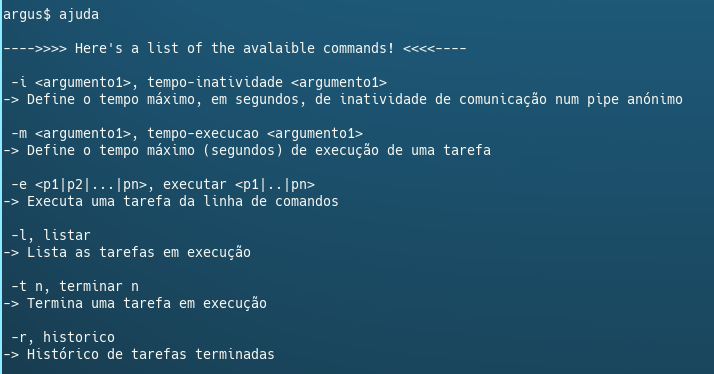
\includegraphics[scale=0.4]{SO7.png}
\caption{Ajuda}
\label{img: Ajuda}
\end{figure}

\subsection{\textbf{Histórico de tarefas}}
Funcionalidade que lista registo historico de tarefas terminadas.
\begin{figure}[H]
\centering
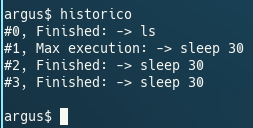
\includegraphics[scale=0.9]{SO92.png}
\caption{Histórico de tarefas}
\label{img: Histórico de tarefas}
\end{figure}

\subsection{\textbf{Terminar tarefas em execução}}
Funcionalidade que termina uma tarefa em execução.
\begin{figure}[H]
\centering
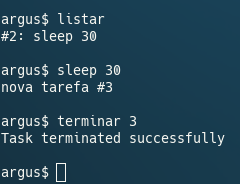
\includegraphics[scale=0.8]{SO91.png}
\caption{Terminar tarefas em execução}
\label{img: Terminar tarefas em execução}
\end{figure}

\pagebreak

\section{Conclusão}
\label{sec:conclusao}
Face ao problema apresentado e analisando criticamente a solução proposta
concluímos que cumprimos as tarefas, conseguindo atingir os objetivos definidos.
De facto, foram implementadas todas as funcionalidades apresentadas, quer
básicas quer avançadas.
Deste modo, foi então construído um sistema de Controlo e Monitorização de Processos e Comunicação
perfeitamente funcional, capaz de executar com exatidão todas as tarefas propostas pelo enunciado deste trabalho prático. 

\end{document}